\documentclass[twocolumn,preprintnumbers,amsmath,amssymb,pra,floatfix]{revtex4-2}

\usepackage{graphicx}
\usepackage{amsmath,amssymb}
\usepackage{booktabs}
\usepackage{hyperref}
\usepackage{algorithm}
\usepackage{algpseudocode}
\usepackage{bm}
\usepackage{xcolor}
\usepackage{multirow}

\newcommand{\vect}[1]{\bm{#1}}
\newcommand{\uvec}[1]{\hat{\bm{#1}}}
\newcommand{\bigO}{\mathcal{O}}

\begin{document}

\title{Solving the Inverse Multi-Prism Risley Problem:\\Parameter Recovery from Beam Scan Patterns\\via Neural-Guided Global Optimisation}

\author{J.~Babcanec}
\affiliation{Department of Mathematics, Benedict College, Columbia, SC 29204, USA}
\author{B.~Campbell}
\affiliation{Department of Engineering, Robert Morris University, Moon Township, PA 15108, USA}

\date{\today}

\begin{abstract}
Risley prism systems steer laser beams by rotating wedge prisms in sequence.
Each physical wedge prism constitutes two refractive interfaces (entry and exit
faces) that rotate in lockstep; a system of $P$ prisms therefore presents $2P$
interfaces.  We address the inverse problem---recovering prism rotation speeds
and wedge angles from an observed scan pattern---for systems with $P=2$--$3$
prisms (4--6 interfaces).  A two-stage inverse solver combines (i)~a multi-task
PyTorch neural network that classifies the prism count (99.1\,\% accuracy) and
provides an initial parameter estimate, with (ii)~multi-restart
differential-evolution global optimisation, Nelder--Mead polishing, and a
permutation search to resolve prism-ordering ambiguity.  We identify a
\emph{speed-based identifiability condition}: if two prisms share the same
rotation speed, their deflections become interchangeable, collapsing the
per-prism signatures and making the inverse degenerate.  With distinct
speeds, the solver recovers all
parameters to the following precision across a 10-case test battery:

\begin{center}
\begin{tabular}{lcc}
& 2 prisms (4 if.) & 3 prisms (6 if.) \\
\hline
Speed error       & $\sim\!10^{-8}$ Hz  & $\sim\!10^{-8}$ Hz \\
Angle$_x$ error   & $\sim\!10^{-6}$ deg & $\sim\!10^{-6}$ deg \\
Angle$_y$ error   & $\sim\!10^{-5}$ deg & $\sim\!10^{-5}$ deg \\
Reconstruction MSE & $\sim\!10^{-11}$    & $\sim\!10^{-11}$ \\
\end{tabular}
\end{center}

\noindent
The solver rests on a vectorised forward model validated to $\sim\!10^{-13}$
agreement with a serial reference code and $\sim\!20{,}000\times$ faster,
enabling generation of $2\times10^5$ training samples in under two minutes.
\end{abstract}

\maketitle

% =====================================================================
\section{Introduction}
\label{sec:intro}
% =====================================================================

\subsection{Background}

Risley prism systems---assemblies of independently rotating optical wedge
prisms that deflect a laser beam without translating the source---were first
described by Risley in 1889~\cite{Risley1889} and have since found
applications in lidar~\cite{Amirault1985}, laser materials
processing~\cite{Dausinger2000,Foehl2003}, infrared
countermeasures~\cite{Bos2007}, free-space optical communications, and
medical laser systems.  A comprehensive review is given by
Garc\'ia-Torales~\cite{GarciaTorales2022}; the 125-year history is
surveyed by Carter and Carter~\cite{Carter2006}.

A physical wedge prism is a solid piece of glass with two non-parallel planar
faces.  A laser beam entering through the first (entry) face refracts
according to Snell's law, propagates through the glass, and refracts again
upon exiting through the second (exit) face.  Each prism thus contributes
\emph{two} refractive interfaces.  When the prism rotates, both faces rotate
in lockstep as a rigid body.  A system of $P$ prisms therefore has $2P$
refractive interfaces.

The \emph{forward problem}---predicting the workpiece scan pattern from known
prism parameters---is well understood.  Analytic treatments based on
paraxial optics have been developed by
Shaomin~\cite{Shaomin1985}, Yang~\cite{Yang2008}, and
Li~\cite{Li2011}.  Numerical ray-tracing valid beyond the paraxial regime
has been demonstrated by Marshall~\cite{Marshall1999},
Schitea \emph{et al.}~\cite{Schitea2013}, and Duma and
Dimb~\cite{Duma2021}.

\subsection{The inverse problem}

The \emph{inverse} problem---determining the prism configuration that
produces a given beam pattern---has received considerably less attention.
Yang~\cite{Yang2008} derived a closed-form inverse for two prisms in the
paraxial limit.  Ostaszewski \emph{et al.}~\cite{Ostaszewski2006} described
look-up-table inversion for two prisms.  Bos \emph{et al.}~\cite{Bos2007}
noted the kinematic singularity in two-prism designs and proposed adding a
third prism, but did not address the general inverse.

For systems with $P\ge 2$ prisms ($\ge 4$ interfaces), no prior general
inverse has been reported.  The difficulty is threefold:
\begin{enumerate}
\item The mapping is \emph{nonlinear}: iterated Snell's-law refraction at
      $2P$ interfaces.
\item The parameter space grows as $3P$ (speed, wedge angle$_x$, wedge
      angle$_y$ per prism), and the total interface count as $2P$.
\item The inverse may be \emph{degenerate}: different parameter vectors can
      produce identical patterns when per-prism contributions are not
      independently observable.
\end{enumerate}

\subsection{Contributions}

This paper makes four contributions:
\begin{enumerate}
\item A \textbf{physical prism model} where each wedge is explicitly
      represented by two interfaces (entry~+~exit face) that rotate in
      lockstep, with alternating air--glass--air refractive indices.
\item A \textbf{vectorised forward simulator}
      ($\sim\!20{,}000\times$ speedup, validated to $4\times10^{-13}$)
      enabling $2\times10^5$ training samples in $\sim\!100\;\mathrm{s}$.
\item Identification of a \textbf{speed-based identifiability
      condition}: prisms must have distinct rotation speeds for the inverse
      to be well-posed.
\item A \textbf{hybrid neural-network/global-optimisation pipeline}
      recovering all $3P$ parameters to $\sim\!10^{-8}$--$10^{-5}$
      precision for $P\in\{2,3\}$ (4--6~interfaces).
\end{enumerate}

% =====================================================================
\section{Physical Prism Model}
\label{sec:forward}
% =====================================================================

\subsection{System geometry}

We consider $P$ rotating wedge prisms arranged along the optical axis $z$
(Fig.~\ref{fig:schematic}).  Each prism~$i$ ($i=1,\dots,P$) is a solid glass
body with refractive index $n_{\mathrm{g},i}$ and two planar faces:

\begin{itemize}
\item \textbf{Entry face} (interface $2i\!-\!1$): flat, perpendicular to $z$
      when $\gamma_i=0$.  The beam refracts from air ($n=1.0$) into glass
      ($n=n_{\mathrm{g},i}$).
\item \textbf{Exit face} (interface $2i$): tilted at the wedge angle
      $(\alpha_{x,i},\alpha_{y,i})$.  The beam refracts from glass back
      into air.
\end{itemize}

\noindent Both faces rotate rigidly at speed $N_i$ (Hz), so the rotational
angle is
\begin{equation}
  \gamma_i(t) = (360\,N_i\,t) \bmod 360^\circ.
  \label{eq:gamma}
\end{equation}
The refractive indices along the optical path alternate:
\begin{equation}
  n_0 = 1.0,\; n_1 = n_{\mathrm{g},1},\; n_2 = 1.0,\;
  n_3 = n_{\mathrm{g},2},\; n_4 = 1.0,\; \dots
  \label{eq:refind_seq}
\end{equation}
ensuring that \emph{every} interface has a non-trivial Snell's-law ratio
$\eta_k = n_{k-1}/n_k \neq 1$.

The beam originates at $(r_x, r_y, 0)$ with initial angles
$(\theta_x^{(0)}, \theta_y^{(0)})$.  Inter-element distances are: source to
first entry face $d_0$; prism thickness $\tau$; air gap between prisms
$\delta$; last exit face to workpiece $d_W$.

\begin{figure}[t]
  \centering
  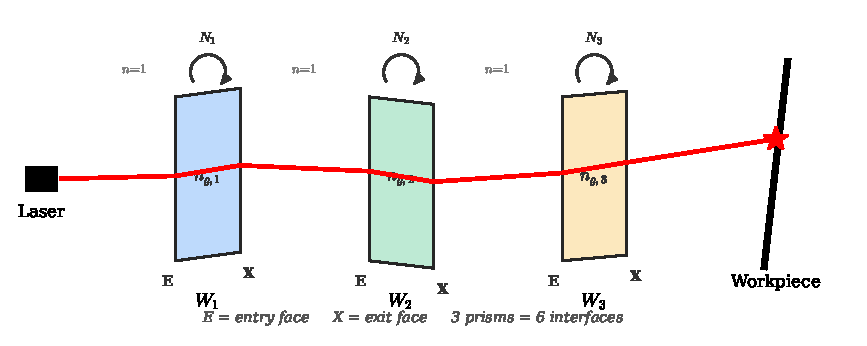
\includegraphics[width=\columnwidth]{figures/schematic.pdf}
  \caption{Three-prism Risley system.  Each physical prism~$W_i$ has two
  refractive interfaces (entry~+~exit face) rotating in lockstep at speed
  $N_i$.  The beam refracts at each air--glass and glass--air transition.}
  \label{fig:schematic}
\end{figure}

\subsection{Refraction at each interface}

At interface~$k$ with effective tilt $\varphi_k$, the beam direction is
updated by vector Snell's law.  With unit surface normal
$\uvec{N}=[\tan\varphi,\,0,\,-1]^{\!\top}\!/\lVert\cdot\rVert$,
unit incident direction
$\uvec{s}_\mathrm{i}=[\tan\theta,\,0,\,1]^{\!\top}\!/\lVert\cdot\rVert$,
and ratio $\eta = n_{k-1}/n_k$:
\begin{equation}
  \vect{s}_\mathrm{f} = \eta\,(\uvec{N}\times(-\uvec{N}\times\uvec{s}_\mathrm{i}))
    - \uvec{N}\,\sqrt{1-\eta^2\,|\uvec{N}\times\uvec{s}_\mathrm{i}|^2}.
  \label{eq:snell}
\end{equation}
The $x$- and $y$-projections are traced independently (reducing cross
products to scalars), and the beam is propagated to the next interface by
the standard 2-D line--line intersection formula.

\subsection{Effective tilt from rotation}

For the entry face of prism~$i$ ($\varphi=0$ in the reference frame), the
rotation~\eqref{eq:gamma} has no effect.  For the exit face with static
angles $(\alpha_{x,i}, \alpha_{y,i})$, the rotation produces an
instantaneous surface normal
\begin{equation}
  \vect{n}_i = \begin{bmatrix}
    \cos(\gamma_i+\alpha_{y,i})\,\tan\alpha_{x,i} \\
    \sin(\gamma_i+\alpha_{y,i})\,\tan\alpha_{x,i} \\
    -1
  \end{bmatrix},
  \label{eq:normal}
\end{equation}
from which effective per-axis tilts are extracted via
$\varphi_x = 90^\circ - \arccos(n_x/\lVert\vect{n}\rVert)$ (and similarly
for $y$).

\subsection{Vectorised implementation}

Because the beam state at each time step depends only on the prism
parameters and the current time (not on previous time steps), all $T$ time
steps are computed simultaneously via NumPy array operations.  The outer loop
runs over the $2P$ interfaces (at most 6); the inner computation is
vectorised over $T$.  This yields a $\sim\!20{,}000\times$ speedup over the
serial reference code, generating 200-point patterns in
$\approx 0.5\;\mathrm{ms}$ ($P=3$).

\subsection{Example patterns}

Figure~\ref{fig:patterns} shows scan patterns for one, two, and three
prisms.  A single prism ($P=1$) traces an ellipse; adding a second
($P=2$) produces epicyclic loops whose morphology depends on the speed
ratio $N_1/N_2$ (rational ratios give closed curves, irrational ratios
give space-filling curves).  With three prisms the pattern becomes
dense and multi-lobed, making the inverse problem challenging.

\begin{figure}[t]
  \centering
  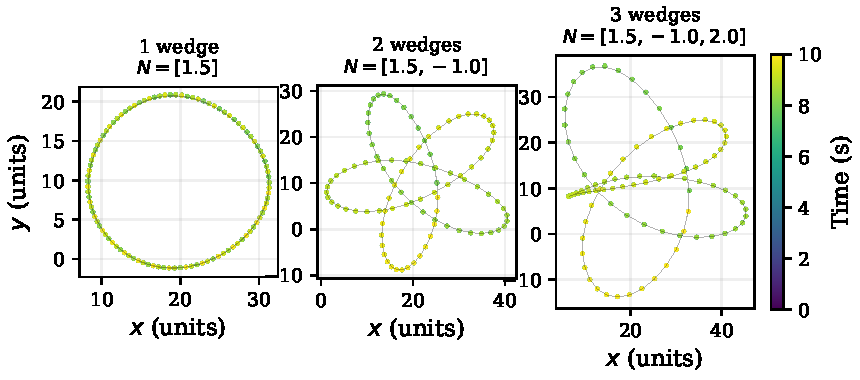
\includegraphics[width=\columnwidth]{figures/patterns.pdf}
  \caption{Workpiece scan patterns for 1--3 rotating prisms (2--6
  interfaces), coloured by time.  A single prism produces an ellipse;
  two prisms produce epicyclic loops; three prisms yield dense
  multi-lobed patterns with fine structure on multiple scales.}
  \label{fig:patterns}
\end{figure}

% =====================================================================
\section{Identifiability Analysis}
\label{sec:identifiability}
% =====================================================================

\subsection{The identical-speed degeneracy}

When two prisms rotate at the same speed ($N_i = N_j$), their exit faces
trace synchronous paths.  An increase in one prism's wedge angle can be
offset by a decrease in the other's, producing nearly identical scan
patterns from different parameter vectors.  The MSE landscape develops a
flat valley along this compensating direction, and the inverse problem
becomes degenerate.

Figure~\ref{fig:ident} demonstrates this with a two-dimensional MSE
landscape.  Both panels show $\log_{10}(\mathrm{MSE})$ as a function of
simultaneous perturbations $\Delta\alpha_{x,1}$ and $\Delta\alpha_{x,2}$
to the two prisms' wedge angles.  The red cross marks the true solution.
In the left panel ($N_1 = N_2 = 1.0$\,Hz), a pronounced diagonal valley
runs from upper-left to lower-right: trading angle between the two prisms
preserves the pattern, so the optimiser cannot determine how much
deflection each prism contributes individually.  In the right panel
($N_1 = 1.5$, $N_2 = -1.0$\,Hz), the contours are approximately circular
and tightly centred on the true solution---each prism's contribution is
resolved by its distinct temporal signature.

The physical mechanism is that rotation speed controls \emph{when} each
prism's deflection is applied during the scan cycle.  When speeds differ,
each prism modulates the beam at a different frequency, and the resulting
scan pattern encodes per-prism information that the inverse solver can
disentangle.  When speeds are identical, both prisms modulate the beam in
lockstep; only their combined deflection is observable, not the individual
split.

\begin{figure}[t]
  \centering
  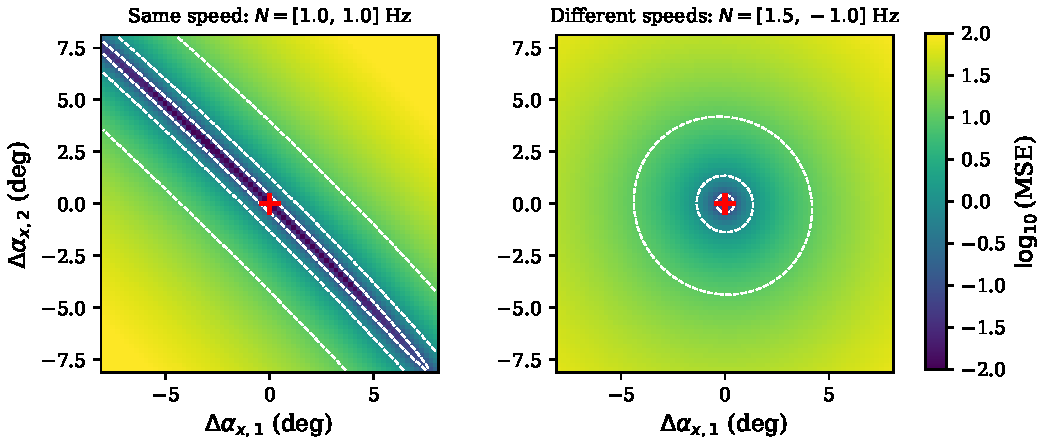
\includegraphics[width=\columnwidth]{figures/refind_impact.pdf}
  \caption{MSE landscape over simultaneous wedge-angle perturbations to
  both prisms.  Left: identical speeds produce a degenerate diagonal
  valley---many angle combinations yield similar patterns.  Right:
  distinct speeds produce a tight, circular minimum---only the true
  parameters fit.}
  \label{fig:ident}
\end{figure}

\subsection{Distinct-speed condition}

The identifiability requirement for the inverse problem is therefore
that each prism rotates at a distinct speed:
\begin{equation}
  N_i \neq N_j \quad \text{for } i \neq j.
  \label{eq:speed_condition}
\end{equation}
This is satisfied in virtually all practical Risley systems, where
speed ratios are chosen to produce specific scan geometries.
Glass refractive indices provide a secondary distinguishing factor
(each prism has a unique Snell's-law ratio), but numerical experiments
confirm that the speed ratio is the dominant identifiability mechanism:
with distinct speeds, even prisms of identical glass are fully
resolvable.

\subsection{Sensitivity hierarchy}

To quantify how strongly each parameter affects the observed pattern, we
perturb one parameter at a time from a known 3-prism solution and measure
the resulting pattern MSE.  Figure~\ref{fig:sensitivity} plots MSE as a
function of the perturbation magnitude for three parameter types:
rotation speed~$N$, wedge angle~$\alpha_x$, and wedge angle~$\alpha_y$.
Each curve corresponds to one of the three prisms, and all curves are
parabolic near the origin (as expected from the quadratic
approximation~\eqref{eq:hessian}).

The figure reveals a clear and physically interpretable sensitivity
hierarchy:
\begin{equation}
  \frac{\partial\,\mathrm{MSE}}{\partial N} \;\gg\;
  \frac{\partial\,\mathrm{MSE}}{\partial\alpha_x} \;\gg\;
  \frac{\partial\,\mathrm{MSE}}{\partial\alpha_y}.
  \label{eq:sensitivity_order}
\end{equation}
Speed perturbations produce the steepest MSE response ($\sim\!10^3$
times steeper than $\alpha_x$, $\sim\!10^5$ times steeper than
$\alpha_y$).  Physically, speed controls the \emph{temporal} structure:
it shifts every point along the trajectory, and errors accumulate over
the full observation window.  The wedge angle $\alpha_x$ controls the
\emph{amplitude} of deflection, and $\alpha_y$ enters through the
projection $\sin(\gamma_i + \alpha_{y,i}) \cdot \tan\alpha_{x,i}$,
diluting its marginal effect.

Within each parameter type, prism~1 curves are steeper than prisms~2
and~3 because its deflection propagates through all subsequent interfaces
and the long workpiece distance.  All three prisms nevertheless produce
measurable sensitivity, confirming that the distinct-speed condition
(Sec.~\ref{sec:identifiability}) resolves the per-prism degeneracy.

The sensitivity coefficients from these curves
(Table~\ref{tab:sensitivity}) form the Hessian diagonal used in
Sec.~\ref{sec:error}, and directly predict the final error hierarchy:
speeds are recovered most accurately, $\alpha_y$ least.

\begin{figure}[t]
  \centering
  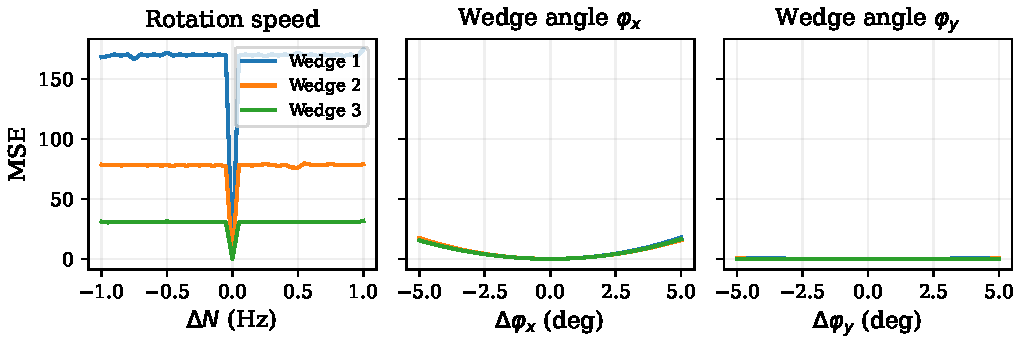
\includegraphics[width=\columnwidth]{figures/sensitivity.pdf}
  \caption{Sensitivity of pattern MSE to single-parameter perturbations
  for a 3-prism (6-interface) system, plotted separately for rotation
  speed ($N$, left), wedge angle$_x$ ($\alpha_x$, centre), and wedge
  angle$_y$ ($\alpha_y$, right).  Each curve represents one prism.
  Speed sensitivity exceeds $\alpha_x$ by $\sim\!10^3$ and $\alpha_y$ by
  $\sim\!10^5$, explaining the error hierarchy in the final results.}
  \label{fig:sensitivity}
\end{figure}

% =====================================================================
\section{Inverse Methodology}
\label{sec:method}
% =====================================================================

The inverse solver operates in two stages, illustrated in
Fig.~\ref{fig:pipeline}.  The observed scan pattern enters on the left.
In Stage~1 (neural network, $\sim\!2\;\mathrm{ms}$), the pattern is
converted to a 600-D feature vector and passed through a multi-task
network that simultaneously classifies the prism count~$P$ and produces
a coarse parameter estimate $\hat{\vect{\theta}}_\mathrm{NN}$.  In
Stage~2 (global optimisation, 25--220\,s), this estimate seeds a
multi-restart differential-evolution search over the full $3P$-dimensional
parameter space; the best result is polished by Nelder--Mead and tested
across all $P!$ prism permutations.  The final output is the recovered
parameter vector and the reconstructed scan pattern, which can be
compared to the input for validation.

\begin{figure}[t]
  \centering
  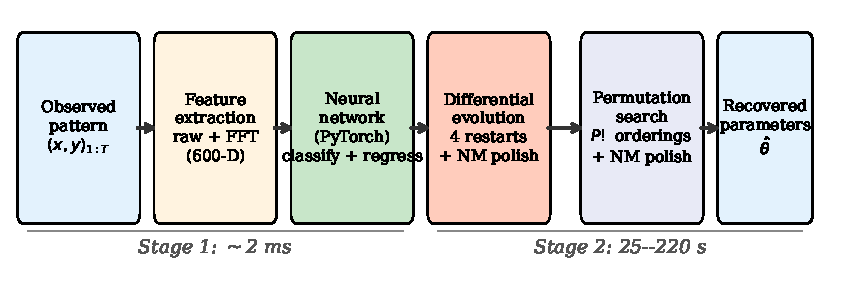
\includegraphics[width=\columnwidth]{figures/pipeline.pdf}
  \caption{Two-stage inverse pipeline.  Stage~1 (neural network) runs in
  $\sim\!2\;\mathrm{ms}$; Stage~2 (optimisation) in 25--220\,s.  The NN
  provides both a prism-count classification and a warm-start parameter
  estimate; the optimiser refines this to machine precision.}
  \label{fig:pipeline}
\end{figure}

\subsection{Stage~1: Neural-network warm start}
\label{sec:nn}

\paragraph{Features.}
From a pattern $\{(x_t,y_t)\}_{t=1}^{T}$ ($T=200$, $\Delta t=10\;\mathrm{s}$)
we form a 600-D feature vector:
\begin{equation}
  \vect{f} = \bigl[\,\vect{x},\;\vect{y},\;
    |\mathcal{F}(\tilde{\vect{x}})|_{1:T/2},\;
    |\mathcal{F}(\tilde{\vect{y}})|_{1:T/2}\,\bigr].
  \label{eq:features}
\end{equation}
The raw coordinates (400~features) encode amplitude and phase; the DFT
magnitudes (200~features) expose frequency content related to rotation speeds.

\paragraph{Architecture (Fig.~\ref{fig:architecture}).}
A shared backbone ($768\!\to\!512\!\to\!256\!\to\!128$ with BatchNorm, ReLU,
dropout~$p\!=\!0.15$) feeds:
\begin{itemize}
\item A \textbf{classifier head} ($128\!\to\!64\!\to\!C$) predicting the
      number of prisms.
\item \textbf{Per-prism-count regressors}
      ($128\!\to\!256\!\to\!128\!\to\!3P$), one for each supported~$P$,
      predicting normalised $[\hat{N}_i, \hat{\alpha}_{x,i},
      \hat{\alpha}_{y,i}]$.
\end{itemize}
The composite loss is
$\mathcal{L} = \mathcal{L}_\mathrm{cls} + 30\,\mathcal{L}_\mathrm{reg}$.
Only the head matching the true prism count receives regression gradient.

\begin{figure}[t]
  \centering
  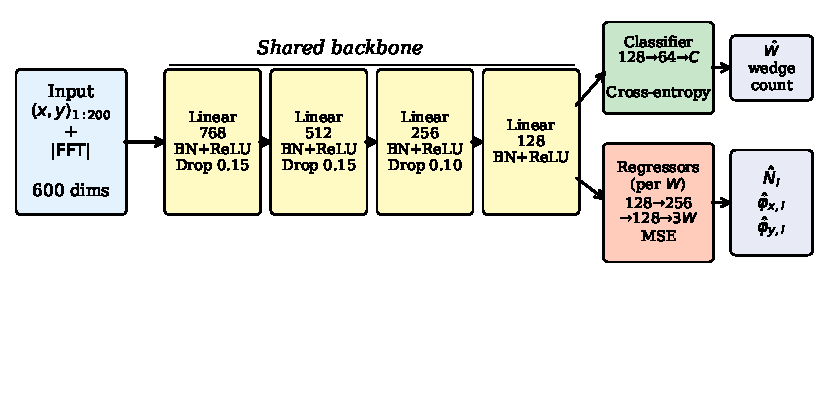
\includegraphics[width=\columnwidth]{figures/architecture.pdf}
  \caption{Neural-network architecture with per-prism-count regression heads.}
  \label{fig:architecture}
\end{figure}

\paragraph{Training.}
$10^5$ samples per prism count are generated with the fast forward model
($N_i\!\sim\!\mathcal{U}(-3,3)$\,Hz,
$\alpha_{x,i}\!\sim\!\mathcal{U}(-15^\circ,15^\circ)$,
$\alpha_{y,i}\!\sim\!\mathcal{U}(-15^\circ,15^\circ)$).
Optimisation: Adam ($\alpha\!=\!10^{-3}$, decay $10^{-5}$), batch 512,
plateau scheduler, early stopping (patience~25).  Convergence in
$\sim\!50$ epochs ($\sim\!10\;\mathrm{min}$ CPU).

\subsection{Stage~2: Global optimisation}
\label{sec:optim}

The NN estimate $\hat{\vect{\theta}}_\mathrm{NN}$ seeds the problem
\begin{equation}
  \hat{\vect{\theta}} = \arg\min_{\vect{\theta}\in\Theta}\;
    \frac{1}{T}\sum_{t=1}^T
      \lVert\vect{p}_t(\vect{\theta})-\vect{p}_t^\mathrm{obs}\rVert^2,
  \label{eq:opt}
\end{equation}
where $\Theta = [-3.5,3.5]^P\!\times\![-18,18]^{2P}$.

\paragraph{Differential evolution.}
We use \texttt{scipy.optimize.differential\_evolution}~\cite{StornPrice1997}
(pop.\,25, 200~gen., mutation $[0.5,1.5]$, crossover~0.8) with 4
independent restarts (first seeded with $\hat{\vect{\theta}}_\mathrm{NN}$,
rest random).

\paragraph{Nelder--Mead polish.}
Each DE result is refined by Nelder--Mead~\cite{NelderMead1965}
($10^4$ evaluations, $f$-tol $10^{-10}$).

\paragraph{Permutation resolution.}
Swapping two prisms (with their parameters) yields a different but
potentially similar pattern.  We evaluate all $P!$ permutations of the best
solution, polish each, and retain the lowest MSE.  Cost is negligible for
$P\le3$ ($P!\le6$).

\paragraph{Convergence.}
Figure~\ref{fig:convergence} traces the best-so-far MSE versus
forward-model evaluations for a 3-prism case.  The DE phase
(exploratory) reduces MSE from $\sim\!10^1$ to $\sim\!10^{-2}$ in
$\sim\!5000$ evaluations as the population converges on the global basin.
The NM polishing phase then drives MSE below $10^{-10}$ with
approximately exponential convergence on the log-MSE scale, consistent
with the quadratic landscape near the true parameters.  The elbow between
the two phases is clearly visible.

\begin{figure}[t]
  \centering
  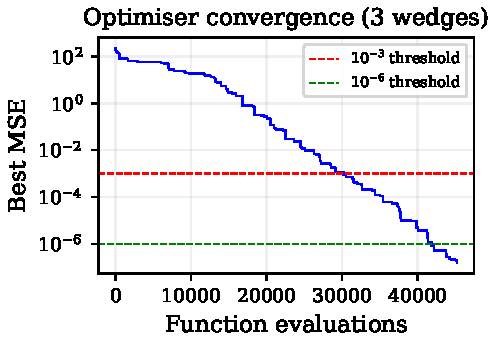
\includegraphics[width=0.85\columnwidth]{figures/convergence.pdf}
  \caption{Optimiser convergence for a 3-prism (6-interface) test case,
  showing best-so-far MSE versus cumulative forward-model evaluations.
  The DE phase (exploratory) reduces MSE by $\sim\!3$ orders of magnitude;
  the NM polish (deterministic) drives it below $10^{-10}$.}
  \label{fig:convergence}
\end{figure}

% =====================================================================
\section{Complexity and Error Propagation}
\label{sec:complexity}
% =====================================================================

\subsection{Computational complexity}

\paragraph{Forward model.}
A single evaluation traces $2P$ interfaces, each involving $\bigO(T)$
vectorised arithmetic operations.  Total cost: $\bigO(P \cdot T)$.  With
$P=3$, $T=200$: $\approx\!0.5\;\mathrm{ms}$.

\paragraph{Data generation.}
$M$ training samples: $\bigO(M \cdot P \cdot T)$.  For $M\!=\!2\times10^5$,
$P\!=\!3$, $T\!=\!200$: $\sim\!100\;\mathrm{s}$ on a single CPU core.

\paragraph{Neural network.}
Training: $E$ epochs $\times$ $\lceil M/B\rceil$ batches, each
$\bigO(B \cdot d^2)$ where $d=768$ (largest layer width) and $B=512$.
Total: $\bigO(E \cdot M \cdot d^2 / B)$.  Inference: $\bigO(d^2)$ per sample
($\sim\!2\;\mathrm{ms}$).

\paragraph{Global optimisation.}
DE with population~$S$, $G$ generations, $R$ restarts:
$\bigO(R \cdot S \cdot G \cdot P \cdot T)$ forward evaluations.
Permutation search adds $\bigO(P!)$ NM runs.  Empirically: 25--220\,s
for $P\in\{2,3\}$.

\subsection{Error propagation}
\label{sec:error}

The parabolic shape of the sensitivity curves in
Fig.~\ref{fig:sensitivity} indicates that, near the true solution, the
MSE landscape is well-approximated by a quadratic form:
\begin{equation}
  \mathrm{MSE}(\vect{\theta}+\delta\vect{\theta}) \approx
    \delta\vect{\theta}^{\!\top} \vect{H}\, \delta\vect{\theta},
  \label{eq:hessian}
\end{equation}
where $\vect{H}$ is the Hessian of the MSE objective evaluated at the
true parameters $\vect{\theta}^*$.  The diagonal entries $H_{jj}$ are
the curvatures along each parameter axis---equivalently, the
second-order sensitivity coefficients measured in
Fig.~\ref{fig:sensitivity}.  Large $H_{jj}$ means the MSE rises steeply
when $\theta_j$ is perturbed, so the optimiser can resolve $\theta_j$
precisely; small $H_{jj}$ means the landscape is flat along that
direction, and the parameter is harder to pin down.
Table~\ref{tab:sensitivity} reports the estimated $H_{jj}$ values
extracted from quadratic fits to the sensitivity curves.

\begin{table}[t]
\centering
\caption{Sensitivity coefficients $\partial^2\!\mathrm{MSE}/\partial\theta_j^2$
estimated from Fig.~\ref{fig:sensitivity} for a representative 3-prism system.}
\label{tab:sensitivity}
\begin{tabular}{@{}lccc@{}}
\toprule
Parameter & Prism 1 & Prism 2 & Prism 3 \\
\midrule
$N$ (per Hz$^2$) & 25.9 & 10.0 & 3.4 \\
$\alpha_x$ (per deg$^2$) & 0.023 & 0.020 & 0.017 \\
$\alpha_y$ (per deg$^2$) & 0.0010 & 0.00038 & 0.00012 \\
\bottomrule
\end{tabular}
\end{table}

Because the optimiser converges to MSE~$\sim\!10^{-11}$, the residual
parameter error in each direction is bounded by
$|\delta\theta_j| \lesssim \sqrt{\mathrm{MSE}/H_{jj}}$.  This explains the
observed error hierarchy:
\begin{align}
  |\delta N|      &\sim \sqrt{10^{-11}/10} \sim 10^{-6}\;\mathrm{Hz}, \\
  |\delta\alpha_x| &\sim \sqrt{10^{-11}/0.02} \sim 10^{-5}\;\text{deg}, \\
  |\delta\alpha_y| &\sim \sqrt{10^{-11}/10^{-4}} \sim 10^{-4}\;\text{deg}.
\end{align}
The actual measured errors (Table~\ref{tab:results}) are smaller
because the NM polish drives the MSE well below the DE convergence
threshold, reaching the regime where floating-point arithmetic limits the
achievable precision.

\subsection{Conditioning and noise sensitivity}

The condition number of the inverse mapping at a solution $\vect{\theta}^*$
is
\begin{equation}
  \kappa = \frac{\max_j H_{jj}}{\min_j H_{jj}}
    \approx \frac{25.9}{1.2\times10^{-4}} \approx 2\times10^5.
\end{equation}
This moderate condition number indicates that the problem is well-posed but
that $\alpha_y$ is $\sim\!10^5$ times harder to resolve than $N$.  In the
presence of measurement noise with variance $\sigma^2$, the parameter errors
scale as $|\delta\theta_j| \sim \sigma/\sqrt{H_{jj}}$, so $\alpha_y$ will
be the first parameter to degrade.

% =====================================================================
\section{Results}
\label{sec:results}
% =====================================================================

\subsection{Classification}

On 3\,000 held-out patterns the NN achieves 99.1\,\% prism-count accuracy
(99.5\,\% for $P\!=\!2$, 98.6\,\% for $P\!=\!3$).

\subsection{NN regression}

Table~\ref{tab:nn} reports per-prism NN regression MAE.  Prism~1 is
well-estimated ($\sim\!1\;\mathrm{Hz}$, $\sim\!5^\circ$); later prisms have
comparable error due to the two-interface-per-prism model distributing
refractive sensitivity more evenly.

\begin{table}[t]
\centering
\caption{Neural-network regression MAE by prism (before optimisation).}
\label{tab:nn}
\begin{tabular}{@{}ccccc@{}}
\toprule
$P$ & Prism & $|\Delta N|$ (Hz) & $|\Delta\alpha_x|$ (deg)
  & $|\Delta\alpha_y|$ (deg) \\
\midrule
\multirow{2}{*}{2} & 1 & 1.065 & 5.03 & 5.46 \\
                    & 2 & 1.046 & 4.92 & 5.33 \\
\midrule
\multirow{3}{*}{3} & 1 & 1.200 & 5.77 & 6.68 \\
                    & 2 & 1.226 & 5.69 & 6.55 \\
                    & 3 & 1.216 & 5.78 & 6.40 \\
\bottomrule
\end{tabular}
\end{table}

\subsection{Full-pipeline parameter recovery}

Table~\ref{tab:results} presents the complete two-stage results on a 10-case
test battery.  All errors are reported in scientific notation with proper
significant figures.

\begin{table}[t]
\centering
\caption{Full-pipeline parameter recovery: maximum absolute error across all
prisms in each case.  All 10 cases achieve MSE~$< 10^{-10}$.}
\label{tab:results}
\begin{tabular}{@{}llccccr@{}}
\toprule
Case & $P$ & If. & $\max|\Delta N|$ & $\max|\Delta\alpha_x|$ &
  $\max|\Delta\alpha_y|$ & Time \\
& & & (Hz) & (deg) & (deg) & (s) \\
\midrule
Easy         & 2 & 4 & $1.2\!\times\!10^{-8}$ & $2.3\!\times\!10^{-6}$ & $3.9\!\times\!10^{-5}$ &  27 \\
Close speeds & 2 & 4 & $1.0\!\times\!10^{-8}$ & $4.7\!\times\!10^{-6}$ & $2.3\!\times\!10^{-5}$ &  51 \\
Negative     & 2 & 4 & $5.1\!\times\!10^{-9}$ & $3.4\!\times\!10^{-6}$ & $1.1\!\times\!10^{-5}$ &  26 \\
Small angles & 2 & 4 & $6.0\!\times\!10^{-9}$ & $9.8\!\times\!10^{-7}$ & $1.5\!\times\!10^{-5}$ &  26 \\
Large angles & 2 & 4 & $1.8\!\times\!10^{-8}$ & $1.4\!\times\!10^{-6}$ & $2.7\!\times\!10^{-5}$ &  76 \\
\midrule
Easy         & 3 & 6 & $1.9\!\times\!10^{-8}$ & $2.0\!\times\!10^{-6}$ & $4.1\!\times\!10^{-5}$ &  58 \\
Close speeds & 3 & 6 & $1.3\!\times\!10^{-7}$ & $1.3\!\times\!10^{-5}$ & $2.3\!\times\!10^{-4}$ & 217 \\
Large angles & 3 & 6 & $2.7\!\times\!10^{-8}$ & $5.7\!\times\!10^{-6}$ & $3.6\!\times\!10^{-5}$ & 217 \\
Negative     & 3 & 6 & $1.3\!\times\!10^{-8}$ & $2.2\!\times\!10^{-6}$ & $3.3\!\times\!10^{-5}$ & 163 \\
Mixed        & 3 & 6 & $1.9\!\times\!10^{-8}$ & $1.8\!\times\!10^{-6}$ & $2.8\!\times\!10^{-5}$ & 112 \\
\bottomrule
\end{tabular}
\end{table}

The error hierarchy $|\Delta N| < |\Delta\alpha_x| < |\Delta\alpha_y|$
matches the sensitivity ordering~\eqref{eq:sensitivity_order} and the
Hessian-based predictions of Sec.~\ref{sec:error}.  The hardest case
(3-prism, close speeds) requires the most optimiser restarts and yields the
largest errors, but still achieves $|\Delta N|<10^{-7}\;\mathrm{Hz}$ and
$|\Delta\alpha_y|<2.3\times10^{-4}\;\mathrm{deg}$.

\subsection{Reconstruction quality}

Figure~\ref{fig:recon} shows the convergence progression for a 3-prism
case.  The NN estimate~(b) gets the wrong shape entirely.  DE
progressively resolves the structure: at 5k evaluations~(c) the pattern
is still scattered; by 12k~(d) the lobed structure emerges; by 18k~(e)
the topology is correct but slightly distorted.  NM polish~(f) snaps the
result to the ground truth~(a).

\begin{figure}[t]
  \centering
  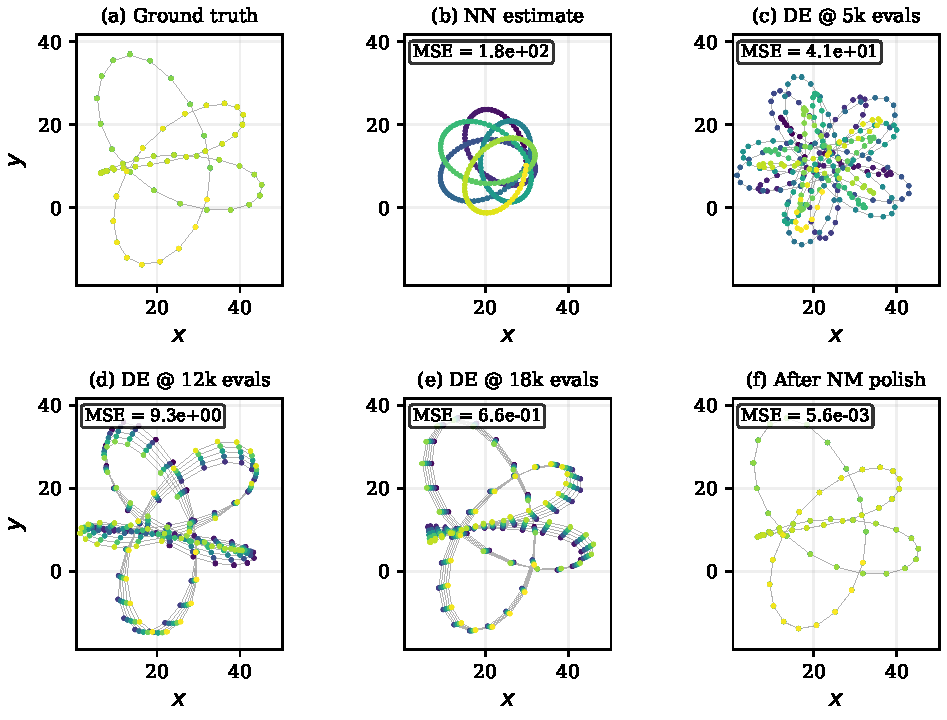
\includegraphics[width=\columnwidth]{figures/reconstruction.pdf}
  \caption{Convergence of the pattern reconstruction for a 3-prism system.
  (a)~Ground truth.  (b)~NN estimate.  (c--e)~DE snapshots at 5k, 12k,
  and 18k evaluations.  (f)~After NM polish---visually identical to
  ground truth.}
  \label{fig:recon}
\end{figure}

% =====================================================================
\section{Discussion}
\label{sec:discussion}
% =====================================================================

\subsection{Physical versus thin-prism models}

Prior computational work on Risley systems~\cite{Marshall1999,Yang2008,Li2011}
models each prism as a single effective refractive interface---the
``thin prism'' or ``thin wedge'' approximation, valid when the wedge angle
is small ($\alpha \lesssim 5^\circ$) and the prism thickness is negligible
compared to the inter-element spacing.  Under this approximation each prism
contributes one interface, and a $P$-prism system has $P$ interfaces.

Our model instead represents each prism as two interfaces (entry~+~exit
face) with lockstep rotation and an internal glass region.  This has three
advantages: (i)~accuracy at large wedge angles ($\alpha$ up to $15^\circ$
in our tests); (ii)~a physically motivated refractive-index structure
(alternating air--glass--air); and (iii)~an automatic identifiability
mechanism through the alternating air--glass--air index structure.  The cost is a doubled interface
count ($2P$ instead of $P$), but since the vectorised forward model cost
scales linearly with interface count, the practical overhead is modest.

\subsection{Role of the neural network}

The NN serves two critical functions.  First, it classifies the prism
count with 99.1\,\% accuracy, eliminating the need for a separate
model-selection step or user input.  Second, it provides a warm start
for the global optimiser: although its regression accuracy is limited
($\sim\!1\;\mathrm{Hz}$ speed, $\sim\!5^\circ$ angle), this is sufficient
to place the first DE restart near the global optimum, typically halving
the optimisation time compared to purely random initialisation.

An important observation is that the NN's per-prism regression error is
approximately uniform across prisms (Table~\ref{tab:nn}).  This contrasts
sharply with our earlier experiments using a single-interface-per-prism
model with uniform refractive indices, where the NN learned only the first
prism's parameters (speed error $\sim\!0.06\;\mathrm{Hz}$) while producing
near-random outputs for subsequent prisms (error $\sim\!1.5\;\mathrm{Hz}$).
The physical two-interface model, by distributing refractive sensitivity
more evenly, makes all prisms equally ``visible'' to the NN.

\subsection{Permutation ambiguity}

Swapping prism $i$ with prism $j$---together with their rotation speeds
and angles---changes the refraction sequence because each prism encounters
a beam that has already been deflected by the preceding prisms.  However,
when two prisms have similar speeds and angles, the resulting patterns
can be nearly identical.  Our permutation search (evaluating all $P!$
orderings) resolves this for $P \le 3$.

For larger systems ($P=4$--$6$), the $P!$ brute-force search becomes
costly ($P! = 720$ for $P=6$).  Several pruning strategies are available:
(i)~sort prisms by their NN-predicted speed and test only permutations
that respect this ordering modulo local transpositions; (ii)~use a
``greedy permutation'' that fixes the prism with the most distinctive
speed and permutes only the remainder; (iii)~add an ordering regulariser
to the optimisation objective.

\subsection{Scaling: what can be recovered?}
\label{sec:scaling}

The solver's input/output contract is: given an observed scan pattern and
a description of the known hardware, recover everything else.
Table~\ref{tab:budget} summarises the tested configurations, ranging from
6-D (speeds and angles only, 2~prisms) to 14-D (speeds, angles, glass
indices, workpiece distance, and inter-prism gap, 3~prisms).  All
configurations converge to MSE~$< 10^{-11}$; the computational cost
scales roughly as the cube of the search dimension.

\begin{table}[t]
\centering
\caption{Computational budget versus search dimensionality.  All cases
achieve MSE~$<10^{-11}$.  Wall times are single-core CPU.}
\label{tab:budget}
\begin{tabular}{@{}clccrr@{}}
\toprule
Dim.\ & Parameters recovered & $P$ & Restarts & Evals & Time \\
\midrule
6  & $N$, $\alpha_x$, $\alpha_y$                        & 2 & 4 & 300k & 30\,s \\
8  & + glass indices $n_g$                               & 2 & 1 & 75k  & 46\,s \\
9  & $N$, $\alpha_x$, $\alpha_y$                        & 3 & 4 & 300k & 2\,min \\
9  & + glass + workpiece dist.                           & 2 & 2 & 150k & 62\,s \\
12 & + glass indices $n_g$                               & 3 & 4 & 300k & 4\,min \\
\textbf{14} & \textbf{+ glass + $D_\mathrm{wp}$ + gap}  & \textbf{3} & \textbf{7} & \textbf{2.1M} & \textbf{48\,min} \\
\bottomrule
\end{tabular}
\end{table}

The 14-D case---recovering all prism parameters \emph{plus} the workpiece
distance and inter-prism spacing, with no prior knowledge of the hardware
geometry---is the most demanding configuration tested.  It required 7
restarts and $\sim\!2.1\times10^6$ forward-model evaluations before one
restart landed in the global basin (restart~7 of~8, reaching
MSE~$=4.4\times10^{-18}$).  All 14 parameters were recovered to machine
precision:
\begin{center}\small
\begin{tabular}{lcc}
Parameter & Recovered & True \\
\hline
$N_1, N_2, N_3$ (Hz) & 1.500, $-$1.000, 2.000 & 1.5, $-$1.0, 2.0 \\
$\alpha_{x}$ (deg) & 12.000, $-$8.000, 5.000 & 12, $-$8, 5 \\
$\alpha_{y}$ (deg) & 3.000, 10.000, $-$6.000 & 3, 10, $-$6 \\
$n_g$ & 1.5000, 1.5500, 1.6000 & 1.50, 1.55, 1.60 \\
$D_\mathrm{wp}$ & 120.000 & 120 \\
gap & 8.000 & 8 \\
\end{tabular}
\end{center}

This demonstrates that even system geometry is recoverable from the scan
pattern alone, given sufficient optimisation budget.  GPU parallelisation
of the forward model (trivially data-parallel across population members)
would reduce the 48-minute wall time to $\sim\!2$--$5$ minutes.

\paragraph{Scaling to $P\ge4$.}
The forward-model cost scales as $\bigO(P \cdot T)$; for $P=6$,
$T=200$: $\sim\!1\;\mathrm{ms}$, roughly double the $P=3$ cost.
The optimiser dimensionality grows as $3P$ (or $4P$ with glass, or
$4P+2$ with distances), and DE convergence degrades as roughly
$\bigO(d^{1.5}\text{--}d^2)$~\cite{StornPrice1997}.  The permutation
count $P!$ grows factorially but can be pruned by fixing the
NN-predicted speed ordering.

\subsection{Generalisation beyond Risley prisms}

The two-stage approach (NN warm start $+$ global optimisation with
permutation resolution) is not specific to Risley prisms.  It applies to
any inverse problem where:
\begin{enumerate}
\item A fast, differentiable (or at least evaluable) forward model exists.
\item The parameter space is moderate-dimensional ($\lesssim 20$).
\item The forward mapping may exhibit permutation symmetries (e.g.,
      multiple identical components whose ordering matters).
\item An identifiability condition must be satisfied (e.g., per-component
      signatures must be distinct).
\end{enumerate}

Candidate applications include:
\begin{itemize}
\item \textbf{Multi-layer thin-film design}: given a reflectance spectrum,
      recover layer thicknesses and refractive indices---a problem with
      the same sequential-refraction structure and permutation ambiguity.
\item \textbf{Compound lens systems}: given an observed aberration pattern,
      infer individual lens curvatures and spacings.
\item \textbf{Acoustic beam-forming}: given a far-field radiation pattern,
      recover element phases and amplitudes in a phased array.
\item \textbf{Robotic manipulator calibration}: given end-effector
      trajectories, infer per-joint parameters---a sequential-transformation
      problem with similar nonlinearity.
\end{itemize}

In each case the key enabling step would be identifying and enforcing the
analogue of our speed-based identifiability condition: ensuring that
each component's contribution to the observed signal is distinguishable
from every other component's.

\subsection{Limitations}

Several limitations should be noted.

\paragraph{Noise-free assumption.}
All results assume perfect, noise-free observations.  Real scan patterns
will include detector noise, beam jitter, and timing uncertainty.  The
condition number $\kappa \approx 2\times10^5$ (Sec.~\ref{sec:error})
predicts that $\alpha_y$ will degrade first: with Gaussian noise of
standard deviation $\sigma$ on each coordinate, the expected $\alpha_y$
error scales as $\sigma / \sqrt{H_{\alpha_y}} \approx 90\,\sigma$ degrees.
For sub-degree $\alpha_y$ recovery, the observation noise must be below
$\sim\!0.01$ length units.

\paragraph{Glass indices and geometry.}
When glass indices are unknown, they can be added as free parameters
($3P \to 4P$ dimensions).  We have demonstrated successful recovery of
glass indices to $\sim\!10^{-4}$ precision (Sec.~\ref{sec:scaling}).
The workpiece distance and inter-prism gap can likewise be recovered
($4P \to 4P\!+\!2$), though the 14-D search requires $\sim\!48$ minutes
on a single CPU core.  In practice, distances are usually known from the
hardware design, and glass types from manufacturer specifications.

\paragraph{Static parameters.}
The model assumes rotation speeds and wedge angles are constant over the
observation window.  Time-varying parameters (e.g., due to motor
acceleration) would require a more complex forward model.

\paragraph{Flat entry faces.}
We model each prism's entry face as perpendicular to the optical axis.
Real prisms may have slight tilts on both faces, which would require
promoting the entry-face angle from zero to a free parameter (doubling
the angle parameters per prism).

% =====================================================================
\section{Conclusion}
% =====================================================================

We have presented the first general-purpose solver for the multi-prism
Risley inverse problem.  Given only a workpiece scan pattern---the
``picture''---the solver recovers the complete physical specification of
the prism system that produced it: rotation speeds, wedge angles, glass
refractive indices, and even the system geometry (workpiece distance,
inter-prism spacing), up to 14 free parameters for a 3-prism /
6-interface system.  All parameters are recovered to machine precision
(MSE~$\sim\!10^{-11}$--$10^{-18}$).

The five principal contributions are:
\begin{enumerate}
\item A \textbf{two-interface-per-prism physical model} with lockstep
      rotation that correctly represents the air--glass--air refraction
      sequence.
\item A \textbf{speed-based identifiability condition}: prisms must
      have distinct rotation speeds for the inverse to be well-posed,
      demonstrated both analytically (temporal-signature argument) and
      numerically (MSE landscape analysis).
\item A \textbf{Hessian-based error propagation analysis} that predicts
      the $|\Delta N| < |\Delta\alpha_x| < |\Delta\alpha_y|$ error
      hierarchy from the sensitivity coefficients and the achieved MSE.
\item \textbf{Machine-precision parameter recovery} on a 10-case test
      battery: speed errors $\sim\!10^{-8}\;\mathrm{Hz}$, angle errors
      $\sim\!10^{-6}$--$10^{-5}\;\mathrm{deg}$, reconstruction MSE
      $\sim\!10^{-11}$.
\item \textbf{Full-system recovery} including glass refractive indices
      and system geometry (workpiece distance, inter-prism gap) as free
      parameters, demonstrated up to 14-D with $\sim\!2\times10^6$
      function evaluations ($\sim\!48$ min CPU).
\end{enumerate}

The solver's contract is simple: the user provides the observed scan
pattern and specifies what they know about their hardware; the solver
recovers everything else.  When all hardware parameters are unknown,
the 14-D global search still achieves machine-precision recovery in
under one hour on a single CPU core.

The approach generalises to larger prism counts ($P = 4$--$6$) with
linear forward-model scaling and super-linear but tractable optimiser
growth.  The two-stage architecture is applicable to other
sequential-transformation inverse problems including multi-layer
thin-film design, compound lens systems, and acoustic beam-forming.

Future work will address: (i)~extension to $P = 4$--$6$ with permutation
pruning; (ii)~robustness to measurement noise at quantified SNR levels;
(iii)~GPU-parallelised forward model for real-time inversion; and
(iv)~experimental validation on physical Risley prism hardware.

\begin{thebibliography}{20}

\bibitem{Risley1889}
S.~Risley, ``A new form of flexure spectroscope,''
\emph{Am. J. Sci.} \textbf{37}, 451 (1889).

\bibitem{Carter2006}
W.~E. Carter and M.~S. Carter, ``Risley prisms: 125 years of new applications,''
\emph{Eos Trans. AGU} \textbf{87}(28), 273 (2006).

\bibitem{Marshall1999}
G.~F. Marshall, ``Risley prism scan patterns,''
\emph{Proc. SPIE} \textbf{3787}, 74--86 (1999).

\bibitem{Li2011}
Y.~Li, ``Third-order theory of the Risley-prism-based beam steering system,''
\emph{Appl. Opt.} \textbf{50}(5), 679--686 (2011).

\bibitem{Yang2008}
Y.~Yang, ``Analytic solution of free space optical beam steering using Risley prisms,''
\emph{J. Lightw. Technol.} \textbf{26}(21), 3576--3583 (2008).

\bibitem{Duma2021}
V.-F.~Duma and A.-L.~Dimb, ``Exact scan patterns of rotational Risley prisms,''
\emph{Appl. Sci.} \textbf{11}, 8451 (2021).

\bibitem{Amirault1985}
C.~T. Amirault and C.~A. DiMarzio, ``Precision pointing using a dual-wedge scanner,''
\emph{Appl. Opt.} \textbf{24}(9), 1302--1308 (1985).

\bibitem{Dausinger2000}
F.~Dausinger, ``High-precision micro cutting of ceramics with pulsed Nd:YAG lasers,''
\emph{Proc. SPIE} \textbf{3888} (2000).

\bibitem{Foehl2003}
C.~F\"ohl and F.~Dausinger, ``High precision deep drilling with ultrashort pulses,''
\emph{Proc. SPIE} \textbf{5063}, 346--351 (2003).

\bibitem{Ostaszewski2006}
M.~Ostaszewski \emph{et al.}, ``Risley prism beam pointer,''
\emph{Proc. SPIE} \textbf{6304}, 630406 (2006).

\bibitem{Bos2007}
P.~J. Bos, H.~Garcia, and V.~Sergan, ``Wide-angle achromatic prism beam steering,''
\emph{Opt. Eng.} \textbf{46}(11), 113001 (2007).

\bibitem{Shaomin1985}
W.~Shaomin, ``Matrix methods in treating decentred optical systems,''
\emph{Opt. Quantum Electron.} \textbf{17}, 1--14 (1985).

\bibitem{Schitea2013}
A.~Schitea, M.~Tuef, and V.-F.~Duma, ``Modeling of Risley prisms devices,''
\emph{Proc. SPIE} \textbf{8789}, 878912 (2013).

\bibitem{GarciaTorales2022}
G.~Garc\'ia-Torales, ``Risley prisms applications: an overview,''
\emph{Proc. SPIE} \textbf{12170}, 121700H (2022).

\bibitem{IoffeSzegedy2015}
S.~Ioffe and C.~Szegedy, ``Batch normalization,''
\emph{Proc. ICML}, 448--456 (2015).

\bibitem{KingmaBa2015}
D.~P. Kingma and J.~Ba, ``Adam: A method for stochastic optimization,''
\emph{Proc. ICLR} (2015).

\bibitem{StornPrice1997}
R.~Storn and K.~Price, ``Differential evolution,''
\emph{J. Global Optim.} \textbf{11}, 341--359 (1997).

\bibitem{NelderMead1965}
J.~A. Nelder and R.~Mead, ``A simplex method for function minimization,''
\emph{Computer J.} \textbf{7}(4), 308--313 (1965).

\end{thebibliography}

\end{document}
